%=============================================================================
% EVALUATION

\documentclass[../mpaper.tex]{subfiles}

\begin{document}

We presented our developed dashboard to real developers, to evaluate its usability using formalised methods and determine its scope in their development process, by carrying out multiple experiments with them (and their teams) in unique circumstances to be able to understand subjective DX \& productivity with a broad sample of participants.

\subsubsection*{Objectives}

The main goal of our implementation was to provide developers with a visual representation of \textbf{realistic} measures that reflect their development activity; these are not limited like objective metrics but include other relevant factors that occur between the discrete commits (such as referring to documentation, writing tests, etc) to elaborate contexts for changes to the codebase. By presenting this information in a clear and concise manner, the dashboard aims to help developers evaluate their task estimation and effectiveness; it also can help identify bottlenecks \& struggling points, which can then be addressed through refactoring and other improvements to enhance the developer experience.

The experiment sought to verify whether these objectives had been achieved by analysing the impact of the dashboard on developer productivity and satisfaction in estimating their future tasks and diagnosing blockers; it also looked to gather insight on the specific metrics that developers were interested and are hoping for.

\subsubsection*{Demographics}

We only recruited people that were software developers, familiar with issue tracking \& version control and additionally working on a real software project (with/without a team) at the same time as the experiment. Aside from the survey we ran on online forums (through Reddit communities and Discord servers), all experiments were conducted in person at the University of Glasgow. The majority of participants were in their twenties, male and completing their Bachelors degree, while the sample also included developers with a Masters degree and/or who do not identify as male. 80\% participants were involved with web development roles, 40\% native apps development, 27\% in DevOps, and 6\% were involved in research. Despite all participants being exposed to version control before, about 85\% of participants used it frequently; most used issue tracking and feature branching disciplines along with occasional coordination by communicating over Discord/Slack/Teams. Almost all of them used Visual Studio Code \& GitHub, along with the usage of self-hosted instances of GitLab. Of participants that used the dashboard for their own projects, 10 were in an agile team who met regularly in person, 1 in a remote agile team and 1 working individually; most of these developers were aspirational recruits as they were learning professional software development through a course at the university. Most did not think much of their current productivity; see \autoref{fig:demographics}.

\begin{figure}
    \centering
    \begin{subfigure}{0.6\linewidth}
    	\centering
        \resizebox{\textwidth}{!}{%
        \begin{tikzpicture}
            \pie[pos={8,0}, text=legend, scale font, explode=0.1, rotate=120,color={Periwinkle, Bittersweet, BurntOrange, ForestGreen}]{66.7/Individual, 6.7/{Team: $\leq 8$, remote}, 26.7/{Team: $\leq 8$, in-person}, 0/{Team: $> 8$}}
        \end{tikzpicture}
        }
    	\caption{Team Structure}
    \end{subfigure}
    \hfill
    \begin{subfigure}{0.35\linewidth}
    	\centering
        \begin{tikzpicture}
        \begin{axis}[
            boxplot/draw direction=y,
            width=1.25\textwidth,
            height=1.5\textwidth,
            xticklabels={},
            yticklabels={-2, -1, 0, 1, 2},
            ymin=0, ymax=5
        ]
        \addplot+ [boxplot prepared={
        lower whisker=2, lower quartile=3,
        median=3, upper quartile=4,
        upper whisker=4},
        black,
        fill=Periwinkle
        ] coordinates {};
        \end{axis}
        \end{tikzpicture}
    	\caption{Project Satisfaction}
    \end{subfigure}
    \vskip\baselineskip
    \begin{subfigure}{\linewidth}
    \resizebox{\linewidth}{!}{%
	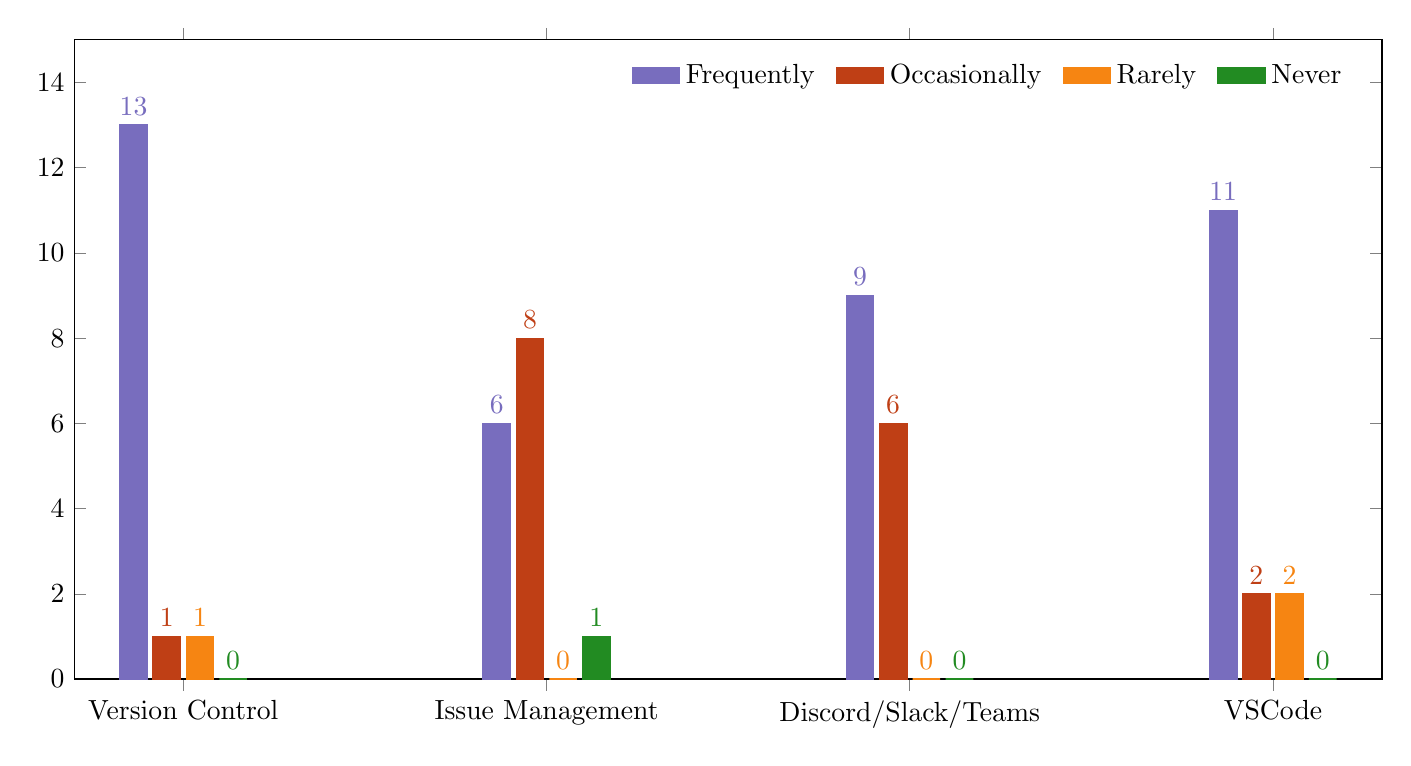
\begin{tikzpicture}
	\begin{axis}[
			ybar,
			% bar width=.5cm,
			width=1.5\textwidth,
			height=.8\textwidth,
			area legend,
            legend style={/tikz/every even column/.append style={column sep=0.2cm},legend columns=5,draw=none},
			symbolic x coords={Version Control, Issue Management, Discord/Slack/Teams, VSCode},
			xtick=data,
			nodes near coords,
			ymin=0,ymax=15,
		]

        % Frequently
		\addplot +[
            Periwinkle
		] coordinates {
			(Version Control, 13)
			(Issue Management, 6)
			(Discord/Slack/Teams, 9)
			(VSCode, 11)
		};

        % Occasionally
		\addplot +[
            Bittersweet
		] coordinates {
			(Version Control, 1)
			(Issue Management, 8)
			(Discord/Slack/Teams, 6)
			(VSCode, 2)
		};

        % Rarely
		\addplot +[
            BurntOrange
		] coordinates {
			(Version Control, 1)
			(Issue Management, 0)
			(Discord/Slack/Teams, 0)
			(VSCode, 2)
		};

        % Never
		\addplot +[
            ForestGreen
		] coordinates {
			(Version Control, 0)
			(Issue Management, 1)
			(Discord/Slack/Teams, 0)
			(VSCode, 0)
		};
  
		\legend{Frequently, Occasionally, Rarely, Never}
  
	\end{axis}
	\end{tikzpicture}
     }
	\caption{Tool usage}
    \end{subfigure}
    \caption{Demographic statistics of participants}
    \label{fig:demographics}
\end{figure}

\subsubsection*{Methodology}

Over the span on 11 weeks, we ran three experiments with the participants to gather results on the effectiveness of our dashboard. These were designed for different conditions on the evaluation nature and ran in parallel to each other.

The first experiment was a longitudinal study to be carried out for 6-8 weeks. It required developers to make use of the dashboard while they work on their projects over sprints and iterations; most worked in teams with other members also participating to generate more data about a team-based project. This experiment had three parts.

\begin{itemize}
    \item \textit{Introduction \& Setup:} After recruitment, developers were provided with an overview of the dashboard and also assisted in getting setup with the extension on the devices they use for development.

    \item \textit{Weekly Feedback:} As the participants worked on their software projects and there was more data available to display on the charts, they were asked to provide feedback on their experience using the dashboard in weekly checkpoints. The feedback form asked them to describe their week of working on their projects, if the dashboard had an effect on their week if there were metrics they were not expecting, and if they had any bug fixes or feature requests to report.

    \item \textit{Retrospective:} At the end of the evaluation period, a retrospective meeting was conducted to study the dashboard with the data collected over the weeks and gather in-depth feedback from the participants on their overall experience with the dashboard.
\end{itemize}

The second experiment aimed to gather impressions and feedback on the dashboard using the industry standard System Usability Scale (SUS). This was designed as an alternative to the longitudinal study allowing developers to participate without their projects and with short commitment (at most 30 minutes). The tasks involved understanding a given project on a high-level and judging the resource allocation by visualising the efforts from the data presented by the dashboard. The sample project chosen for study, "\textit{Portion Mate}\noteurl{https://github.com/ineshbose/portion-mate}", was from our early projects for which we were already using the required technologies such as GitHub \& WakaTime, with strict issue tracking and kanban boards, allowing sufficient data to be provided for the dashboard visualisations. The survey included an project exploratory pre-activity aimed to help participants get context and a sense of the project to understand the visualisations better. % it also helped gain insight into how different developers navigate through information on GitHub.

The third experiment was an online survey helping our results to be accurate by reaching developers around the world. This survey asked developers about their perceptions of Developer Experience \& Productivity by asking if they are conscious of project frustration, the metrics they use in their development, and the priority given in considering DX in their codebase. The survey only aimed to take 5-8 minutes to complete to be respectful of online participants' time, but they were also given the option to use the extension themselves for their projects and provide feedback.

\subsubsection*{Results}

We were unable to gather formal results from the longitudinal evaluation and online survey as we faced time constraints and incomplete participation, however the usability survey reached completion and was able to provide insight. The responses from the ten SUS statements are based on a Likert scale -- a five-point range from Strongly disagree (1) to Strongly agree (5) with 3 being neutral -- and are used to determine a usability score for the system. The statements vary in describing the system as positive (denoted by +) or negative (denoted by -), so inverting the meaning of questions ensures that participants do not lose focus. The usability score is calculated using the following formula:

\[
    \left(\sum_{i=1}^{10} S_{i}\right) \times 2.5
    \quad \quad
    \begin{matrix}
    % 1 \leq  r_{i} \leq 5 \hfil\phantom{000000000000000000000} \\
    S_{i}\begin{cases}
    r_{i} - 1 & \text{\scriptsize if positive ($i$ \% 2 > 0)}\\
    5 - r_{i} & \text{\scriptsize if negative ($i$ \% 2 = 0)}
    \end{cases}
    \end{matrix}
\]

\vskip\baselineskip
\noindent where $i$ is the statement number, $S_{i}$ is a statement, and $r_{i}$ is the scale position for the response to $S_{i}$. The scores can be seen in \autoref{fig:participant_scores} along and the responses spread in \autoref{fig:statement_responses}.

% To get the usability score, the number mapped to the response for each statement (depending if the statement is negative\textsuperscript{-}, then the number is subtracted from 5 i.e. $5 - x$ or if it is positive\textsuperscript{+}, then 1 is subtracted from the number i.e. $x - 1$) added together for each participant, then multiplied by 2.5 % and since the survey used 9 questions instead of 10, divided by 0.9.

% In the short time-frame, while there were incomplete and/or insignificant results, we found some interesting data that will be shared in discussion.
In addition, we conducted short verbal interviews with the developers involved in the longitudinal experiment to gather their feedback; transcriptions are listed in \autoref{fig:interview_responses}. % Did not re-open online survey to generate results from 4 responses

\begin{figure}
	\centering
    \resizebox{0.48\textwidth}{!}{%
	\begin{tikzpicture}
	\begin{axis}[
			xbar stacked,
			area legend,
			legend style={
                /tikz/every even column/.append style={column sep=0.2cm},
				at={(xticklabel cs:0.5)},
				anchor=north,legend columns=5,
				draw=none,font=\footnotesize,
			},
			ytick=data,
			tick label style={font=\footnotesize},
			width=0.8\textwidth,
			% xticklabel={\pgfmathparse{\tick}\pgfmathprintnumber{\pgfmathresult}\%},
			bar width=6mm,
			y dir=reverse,
			yticklabels={%
				Statement 1\textsuperscript{+},%
				Statement 2\textsuperscript{-},%
				Statement 3\textsuperscript{+},%
				Statement 4\textsuperscript{-},%
				Statement 5\textsuperscript{+},%
				Statement 6\textsuperscript{-},%
				Statement 7\textsuperscript{+},%
				Statement 8\textsuperscript{-},%
				Statement 9\textsuperscript{+},%
				Statement 10\textsuperscript{-},%
			},
			xmin=0,
			xmax=15,
            % grid style={line width=.01pt},
		]
		% Strongly disagree
		\addplot[Maroon,fill=Maroon,
			postaction={
				pattern=vertical lines
		}] coordinates
		{(0,0) (1,1) (0,2) (6,3) (0,4) (7,5) (0,6) (5,7) (0,8) (4,9)};
		
		% Disagree
		\addplot[YellowOrange,fill=YellowOrange,
			postaction={
				pattern=horizontal lines
		}] coordinates
		{(1,0) (12,1) (1,2) (5,3) (1,4) (7,5) (1,6) (5,7) (1,8) (4,9)};
		
		% Neutral
		\addplot[Goldenrod,fill=Goldenrod,
			postaction={
				pattern=grid
		}] coordinates
		{(3,0) (2,1) (3,2) (1,3) (3,4) (1,5) (2,6) (3,7) (6,8) (5,9)};
		
		% Agree
		\addplot[YellowGreen,fill=YellowGreen,
			postaction={
				pattern=north east lines
		}] coordinates
		{(5,0) (0,1) (9,2) (2,3) (5,4) (0,5) (6,6) (2,7) (4,8) (2,9)};
		
		% Strongly agree
		\addplot[ForestGreen,fill=ForestGreen,
			postaction={
				pattern=north west lines
		}] coordinates
		{(6,0) (0,1) (2,2) (1,3) (6,4) (0,5) (6,6) (0,7) (4,8) (0,9)};
		
		\legend{Strongly disagree,Disagree,Neither,Agree,Strongly agree}
	\end{axis}
	\end{tikzpicture}
     }
	\caption{Responses for each statement}\label{fig:statement_responses}
\end{figure}

\begin{table}
\centering
\setlength{\tabcolsep}{10pt}
\renewcommand{\arraystretch}{1.5}
\begin{tabular}{|p{3.2cm}|p{1.4cm}p{1.4cm}|}
\hline
                        & \multicolumn{2}{c|}{\textbf{Score}} \\ \hline
\rowcolor[HTML]{EFEFEF} 
\textbf{Participant 1}  & 65.0              & C              \\
\textbf{Participant 2}  & 92.5              & A+              \\
\rowcolor[HTML]{EFEFEF} 
\textbf{Participant 3}  & 72.5              & B-              \\
\textbf{Participant 4}  & 40.0              & F                \\
\rowcolor[HTML]{EFEFEF} 
\textbf{Participant 5}  & 80.0              & A-              \\
\textbf{Participant 6}  & 75.0              & B              \\
\rowcolor[HTML]{EFEFEF} 
\textbf{Participant 7}  & 85.0              & A+              \\
\textbf{Participant 8}  & 72.5              & B-              \\
\rowcolor[HTML]{EFEFEF} 
\textbf{Participant 9}  & 67.5              & C              \\
\textbf{Participant 10} & 87.5              & B+              \\
\rowcolor[HTML]{EFEFEF} 
\textbf{Participant 11} & 60.0              & D              \\
\textbf{Participant 12} & 70.0              & C              \\
\rowcolor[HTML]{EFEFEF} 
\textbf{Participant 13} & 72.5              & B-              \\
\textbf{Participant 14} & 82.5              & A              \\
\rowcolor[HTML]{EFEFEF} 
\textbf{Participant 15} & 85.0              & A+              \\ \hline
\rowcolor[HTML]{E0E0E0} 
{\scriptsize\textbf{Usability Score} (Mean)}        & \textbf{73.83}     & \textbf{B-}     \\ \hline
\end{tabular}
\caption{SUS Score for each participant}\label{fig:participant_scores}
\end{table}

\begin{figure}
    \centering
    \begin{tikzpicture}
    \begin{axis}[
    % ytick={1,2,3},
    width=1.15\linewidth,
    height=0.5\linewidth,
    yticklabels={},
    % nodes near coords,
    ]
    \addplot+ [
    boxplot prepared={
    lower whisker=60, lower quartile=70,
    median=73.75,
    upper quartile=85, upper whisker=92.5,
    },
    black, fill=Goldenrod,
    ] coordinates {};
    \end{axis}
    \end{tikzpicture}
    \caption{SUS Score Distribution}
    \label{fig:score_distribution}
\end{figure}

\begin{figure*}
    \centering
    \begin{subfigure}{0.4\textwidth}
        \centering
        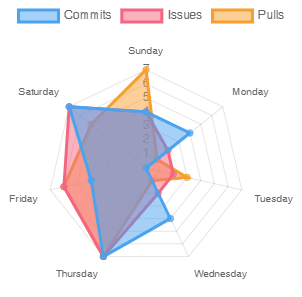
\includegraphics[width=0.7\textwidth]{Screenshot_13-04-radar.png}
        \caption{Displayed graph for sample project}
    \end{subfigure}
    \hfill
    \begin{subfigure}{0.55\textwidth}
        \centering
        \def\arraystretch{1.5}
        \resizebox{1.02\textwidth}{!}{%
        \begin{tabular}{p{0.9\textwidth}}
        \hline
        \textbf{Question:} How would you describe a week for this project?\\ \hline\rowcolor[HTML]{EFEFEF}
        Monday: Commits$^{-}$ (9); "\textit{catch-up}" (1) \\
        Tuesday: Commits (2); Issues (1); Pulls$^{-}$ (3); "\textit{research}" (1) \\\rowcolor[HTML]{EFEFEF}
        Wednesday: Commits$^{-}$ (9); Issues (1); "\textit{work on issues}" (1) \\
        Thursday: Commits$^{+}$ (13); Issues$^{+}$ (13); Pulls (6) \\\rowcolor[HTML]{EFEFEF}
        Friday: Commits (6); Issues (11); Pulls$^{\sim}$ (4) \\
        Saturday: Commits$^{+}$ (12); Issues$^{+}$ (15); Pulls (4) \\\rowcolor[HTML]{EFEFEF}
        Sunday: Commits (5); Issues$^{+}$ (5); Pulls$^{+}$ (12)
        \\ \hline
        \end{tabular}
        }
        \caption{Grouped responses (out of 15)}
    \end{subfigure}
    \caption{Interpretation of the week-radar graph}
    \label{fig:week_radar_resp}
\end{figure*}

\begin{table}
\centering
\def\arraystretch{2}
\resizebox{0.48\textwidth}{!}{%
\begin{tabular}{p{0.5\textwidth}}
\hline
\textbf{Question:} You were one of the developers who was asked to use the dashboard for a few weeks with your project. How would you say your experience was and influence on productivity?\\ \hline\rowcolor[HTML]{EFEFEF}
It was useful in someways with the provided statistics.. not something I'd opening everyday, but once a week to help me remember. The data it provided for our project was pretty useful. If I were to begin again, I would be more efficient.\\
I didn’t find it useful.. I would see GitLab which has nice charts there.. for estimations, we had things like planning poker and 5 whys.. I was already happy with my productivity.\\\rowcolor[HTML]{EFEFEF}
Found it really helpful.. we spent a lot of time on documentation.. it would help my productivity if it was integrated with the project early on.\\
I find it interesting being able to see (more details about) the changes I made.. in general we’re not good at remembering how long we spent on things.. if I was asked later and I didn’t have the data in front of me, I wouldn’t be sure.\\\rowcolor[HTML]{EFEFEF}
Confusing at first, but a week later, it helped me personally, seeing the data.. I mainly use VSCode; I don’t open GitLab, so its helpful than opening another tab for these metrics.\\ \hline % I would be interested in seeing wiki metrics as we always update the wiki.
 % footer \\ \hline
\end{tabular}
}
\caption{Interview responses from developers}
\label{fig:interview_responses}
\end{table}

\begin{table}
\def\arraystretch{1.5}
\begin{tabular}{l|lll}
\hline
              & Not Once & Just One & Two-three times \\ \hline % Upto five times & More than five times
\rowcolor[HTML]{EFEFEF}13/02 - 19/02 & 2        & 1        & 1               \\
20/02 - 26/02 & 1        & 0        & 2               \\
\rowcolor[HTML]{EFEFEF}27/02 - 05/03 & 2        & 4        & 5               \\
06/03 - 12/03 & 2        & 2        & 0               \\
\rowcolor[HTML]{EFEFEF}13/03 - 19/03 & 2        & 3        & 3               \\ \hline
% 20/03 - 26/03 & 0        & 0        & 1               \\ \hline
\end{tabular}
\caption{Frequency of Dashboard Usage over weeks}
\label{fig:dashboard_usage}
\end{table}

\subsubsection*{Discussion}

Some experiments required quick adjustments or changes to be made last minute to the dashboard such as improving sanitisation for Git remote URL, readability in different VSCode themes, and integrating plugins in Unix environments. A key adjustment required to be made was developing a plugin that interacts with a private GitLab instance as participants' repositories were hosted there; this was developed in no more than two days using the same logic as the GitHub plugin and providing the same API required by the core module hence verifying that the modular architecture was achieved, and all revisions or additions to the code were building and deploying to the extension marketplace without issues - the implementation was successful.

Our main metric, the (system) usability score, came to be 73.8 with the corresponding grade as B- which means that the dashboard was an acceptable (to use) product; however, the score for each participant shows great variance (see \autoref{fig:participant_scores,fig:score_distribution}) ranging from 40.0 to 92.5, with a standard deviation of 13, indicating that the user experience for developers using the system was very different and inconsistent. We explain this through the spread in \autoref{fig:statement_responses}.

While 11 participants (73\%) agree to thinking that they would use this system frequently (statement 1), 3 (20\%) feel neutral or unclear about it and one participant (6.7\%) disagrees; they shared that the remoting hosting service already provides graphs (second response in \autoref{fig:interview_responses}) despite using objective metrics. In comparison, these services have developed such graphs over many years and they do not plot large breakdowns on one chart which is efficient in rendering/interaction and understanding for users. However, no participant found the dashboard to be unnecessarily complex (statement 2) except for two participants (13.3\%) who felt neutral about it; this may be because of their demographic that indicates occasional/rare use of version control and working individually more than in-teams.

There was still 73\% agreement in the participants finding the system easy to use (statement 3), and the one disagreeing response uses version control less than frequently so the dashboard may have been difficult to understand in the context of the repository and revisions; in such cases, 20\% of participants felt that they would need the support of a technical person to use the dashboard (statement 4). It can be noted that the metrics are new and overwhelming compared to traditional visualisations provided by current solutions; so we think a short tutorial may be helpful on the first launch showing the user where things are and how they can interact with data. 73\% participants also agree to finding the various functions in the tool well-integrated (statement 5) with one participant disagreeing; this may be in terms of functionality, application or corresponding the right data, however participants did not see any inconsistency in the dashboard (statement 6); this may be biased since they were externally judging a sample project, but the responses also include participants from the longitudinal study.

There is a higher agreement among participants (80\%) as being able to see the dashboard to be understood and used by most people very quickly (statement 7), but the benefit may not be seen by the remaining 20\% as they, again, also do not frequently use version control so they would not have any need. While more than 50\% participants did not find the system to very cumbersome to use (statement 8), there are about a third of the participants either felt neutral or indeed found it difficult to use; the reason for this is likely due to complex graphs, developed in the short-time, presented for an irrelevant project; this is evident in when 46.7\% of participants did not feel very confident using the system (statement 9) as they are introduced to a new interface showing data for a new project that they did not work on and invest in personally to be able to judge the efforts. A similar 50/50 spread is with participants feeling like they needed to learn a lot of things to understand the dashboard (statement 10) with 53.4\% participants disagreeing; this may also be biased as it includes participants from the longitudinal study who went had already gone through the learning curve, but on doing so, they realise the impact of the dashboard as they used it overtime (see all of \autoref{fig:interview_responses}, including the last response to demonstrate the learning curve).

We further verify developers' understanding of the visualisations through \autoref{fig:week_radar_resp} sharing an example of how developers interpreted the graph used to answer a required question in which they had to identify work tasks (commits, issues and PRs) distributed over the week. Almost all participants were able to identify that the majority of the work was done later in the week recognising Thursday as "the most active day". Some responses contained quantifying adjectives that were positive (like "commits were \textit{mainly/mostly/especially frequent} on Saturday", denoted by +), negative ("\textit{some/somewhat/few} pulls on Tuesday", denoted by -), and uncertain ("pulls \textit{potentially} on Friday", denoted by $\sim$). A participant also inferred that the developers' week "\textit{start with a catch-up, setup and research}" on the project; this demonstrates that developers could pick up information differently, some more than others. Similarly, we asked the developers to provide speculation on \href{https://github.com/ineshbose/portion-mate/pull/140}{a large PR of 142 commits} being made in a short-time based on the metric by the dashboard; after investigating through the breakdown, they were able to spot that all previous changes were made on the \texttt{develop} branch and finally being merged for release.

During our longitudinal study, we asked developers at the end of every week using the dashboard if they sought to introduce changes in their process after reflecting on their efforts for the week. Most responses did not share any intentions mostly because 1) there wasn't enough activity data at first, 2) the generated data wasn't anything that they were profoundly unexpecting, and 3) their projects were at the last iteration so changes would be too late, but some developers were able to notice the quality of their commits and inconsistency of work. Rather, they were more motivated to break down commits further and be pushing changes more frequently. We see through the positive responses in \autoref{fig:interview_responses} and the distribution of participants using the dashboard each week \autoref{fig:dashboard_usage} (regardless of participant drop or spike) that some developers picked up on the importance and the applications of such metrics opening the dashboard more than two times during the week (rather than everyday as pointed by the first response in \autoref{fig:interview_responses}). This reveals the overall themes from our result as being able to 1) give an overview of how developers and teams are performing with insight on that behaviour, 2) increase commit frequency, and most importantly, 3) enable self-awareness.

We point out and acknowledge the limitations of our experiments in generating significant results; these include factors such as short timeframe, convenience sampling, and rushed implementation of our tool. We address these further in the next section with plans for improvements.

\end{document}
